\section{Functions}

\subsection{What is a function?}

\begin{figure}[H]
    \centering
    \begin{tikzpicture}
        \draw[rounded corners] (-3, 0) rectangle (-1, -4) {};
        \draw[rounded corners] (1, 0) rectangle (3, -4) {};

        \foreach \i  in {1,...,3} {
            \node[align=center, anchor=center] at (-2, -\i) {\(x_{\i}\)};
        }

        \foreach \i  in {1,...,3} {
            \node[align=center, anchor=center] at (2, -\i) {\(y_{\i}\)};
        }

        \draw[-Latex, very thick, BrickRed] (-1.75, -1) -- (1.75, -1) node[pos=0.5, anchor=south] {\(f\)};

        \draw[-Latex, very thick, BrickRed] (-1.75, -2) -- (1.75, -2);

        \draw[-Latex, very thick, BrickRed] (-1.75, -3) -- (1.75, -2.2);

        \node[anchor=north] at (-2, -4) {Domain \(X\)};

        \node[anchor=north] at (2, -4) {Codomain \(Y\)};

        \draw[rounded corners, MidnightBlue, dashed, thick] (1.25, -0.5) rectangle (2.75, -2.5) {};

        \node[anchor=west, MidnightBlue, align=left] at (3, -1.5) {Image};
        
    \end{tikzpicture}
    \caption{A function, its domain, its codomain and its image.}
    \label{fig:Ch3-function}
\end{figure}

Let \(X\) and \(Y\) be sets. Suppose we have a rule \(f\) that assigns (or ``maps'') each element \(x \in X\) to a unique element \(y \in Y\). This is called a \textit{function} or \textit{mapping}, and is notated as \(y = f(x)\) and \(f : X \rightarrow Y\). The set \(X\) is known as the \textit{domain} of \(f\) while \(Y\) is the \textit{codomain} of \(f\). This is illustrated in figure \ref{fig:Ch3-function}.

We also define the \textit{image} of \(f\) as \(\{y \in Y : \exists x \in X, f(x) = y\}\). Plainly put, the image of a function is the set of all its possible outputs. This is shown in blue in the above diagram.

Note that it is not necessary for all the elements in the codomain to also be elements of the image. Referring back to the diagram, there is no input in \(X\) that could possibly result in the output \(y_3\). In other words, \(y_3\) is in the codomain of \(f\), but not in its image.


\subsection{Total and partial functions}

Consider the function \(f(x) = \sqrt{x}\). Both its domain and codomain are the set of real numbers, i.e. \(f : \mathbb{R} \rightarrow \mathbb{R}\).

Except not really: The function only accepts non-negative numbers as inputs. This kind of function, where it's only defined on a subset of its domain, is called a \textit{partial function}. The opposite of a partial function is a \textit{total function}, which is defined for all elements in its domain.

\begin{figure}[H]
    \centering
    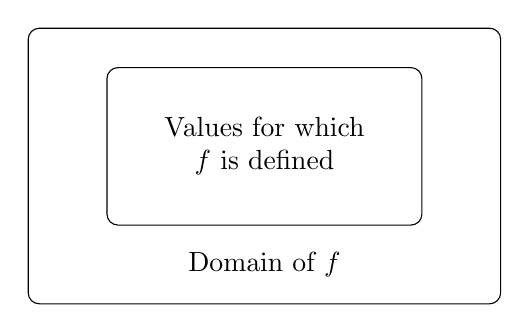
\begin{tikzpicture}
        \draw[rounded corners] (-2,0) rectangle (2,-2);

        \draw[rounded corners] (-3,0.5) rectangle (3,-3);

        \node[align=center] at (0,-1)  {Values for which\\ \(f\) is defined};

        \node[align=center] at (0,-2.5)  {Domain of \(f\)};
    \end{tikzpicture}
    \caption{A partial function \(f\) is only defined for a subset of its domain.}
    \label{fig:ch3-partial-function-maths}
\end{figure}

This distinction between total and partial functions can be generalized to the functions we see in code. For example, consider the following function written in C.
%
\begin{quote}
\begin{verbatim}
int func(int x) {
    do {
        x *= 2;
    } while (!x);
    
    return x;
}
\end{verbatim}
\end{quote}
%
Here, \verb|func| accepts an \verb|int| as input, multiplies it by 2, and returns the product as output. There's just one exception: if we execute the function with input \verb|x = 0|, the function would spiral into an infinite loop without ever producing an output. In other words, the program does not \textit{terminate}.

\begin{table}[H]
    \centering
    \begin{tabular}{|c|c|}
        \hline
        \textbf{Input} & \textbf{Output}\\
        \hline
        -2 & -4 \\
        \hline
        -1 & -2 \\
        \hline
        0 & \textit{(Infinite loop)}\\
        \hline
        1 & 2\\
        \hline
        2 & 4\\
        \hline
    \end{tabular}
    \caption{Examples of inputs and outputs for the \texttt{func} function.}
    \label{tab:ch3-func-input-and-output}
\end{table}

This means that \verb|func| is a partial function: its domain is all values of type \verb|int|, but it only terminates for non-zero inputs.

\begin{figure}[H]
    \centering
    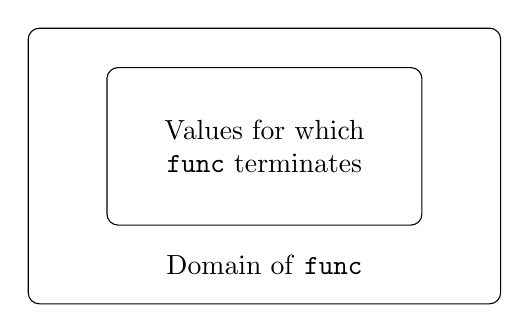
\begin{tikzpicture}
        \draw[rounded corners] (-2,0) rectangle (2,-2);

        \draw[rounded corners] (-3,0.5) rectangle (3,-3);

        \node[align=center] at (0,-1)  {Values for which\\ \texttt{func} terminates};

        \node[align=center] at (0,-2.5)  {Domain of \texttt{func}};
    \end{tikzpicture}
    \caption{A partial function \texttt{func} only terminates for input values from a subset of its domain.}
    \label{fig:ch3-partial-function-cs}
\end{figure}

As a sidenote, it is impossible for an algorithm to take a function as an input and determine whether that function terminates or not. This is known as the \textit{halting problem} (or \textit{entscheidungsproblem}). In 1936, Alan Turing proved that the halting problem is generally undecidable.


\subsection{Seqential composition of functions}

Consider the functions \(f : X \rightarrow Y\) and \(g : Y \rightarrow Z\).

In mathematics, we can create a composition of these two functions \(h(x) = g(f(x))\), where \(h : X \rightarrow Z\). Here, we first apply \(f\) to the input value, and then apply \(g\) to give the output. This is denoted as
%
\[h = g \circ f\text{.}\]
%
Notice how the function that is applied first (\(f\)) is written on the right.

In computer science, we can similarly define the composition of two functions in accordance with the sequential composition paradigm. We use the following notation.
%
\[h = f; g\]
%
where the functions are written in the order in which they are applied. A semicolon is used to separate the composited functions, similar to how we use semicolons to separate consecutive statements in many programming languages.


\subsection{Injections (encodings)}

A function \(f : X \rightarrow Y\) is \textit{injective} if
%
\[\forall a, b \in X,\; f(a) = f(b) \Rightarrow a = b\]
%
or
%
\[\forall a, b \in X,\; a \neq b \Rightarrow f(a) \neq f(b)\text{.}\]
%
These two definitions are contrapositives of each other and are thus equivalent. An injective function is called an \textit{injection} or an \textit{encoding}.

\begin{figure}[H]
    \centering
    \begin{tikzpicture}
        \draw[rounded corners] (-3, 0) rectangle (-1, -4) {};
        \draw[rounded corners] (1, 0) rectangle (3, -4) {};

        \foreach \i  in {1,...,3} {
            \node[align=center, anchor=center] at (-2, -\i) {\(x_{\i}\)};
        }

        \foreach \i  in {1,...,3} {
            \node[align=center, anchor=center] at (2, -\i) {\(y_{\i}\)};
        }

        \draw[-Latex, very thick, BrickRed] (-1.75, -1) -- (1.75, -1) node[pos=0.5, anchor=south] {\(f\)};

        \node[anchor=north, BrickRed, align=left] at (0, -5) {\textbf{Not injective}};

        \draw[-Latex, very thick, BrickRed] (-1.75, -2) -- (1.75, -2);

        \draw[-Latex, very thick, BrickRed] (-1.75, -3) -- (1.75, -2.2);

        \draw[MidnightBlue, very thick, dashed] (2,-2) circle [radius=0.5];

        \node[anchor=north] at (-2, -4) {Domain \(X\)};

        \node[anchor=north] at (2, -4) {Codomain \(Y\)};

        \draw[thick] (4, 1) -- (4, -6);
        
        \begin{scope}[shift={(8, 0)}]
            \draw[rounded corners] (-3, 0) rectangle (-1, -4) {};
            \draw[rounded corners] (1, 0) rectangle (3, -4) {};
    
            \foreach \i  in {1,2} {
                \node[align=center, anchor=center] at (-2, -\i) {\(x_{\i}\)};
            }
    
            \foreach \i  in {1,...,3} {
                \node[align=center, anchor=center] at (2, -\i) {\(y_{\i}\)};
            }
    
            \draw[-Latex, very thick, ForestGreen] (-1.75, -1) -- (1.75, -1) node[pos=0.5, anchor=south] {\(g\)};

            \node[anchor=north, ForestGreen, align=left] at (0, -5) {\textbf{Injective}};
            
            \draw[-Latex, very thick, ForestGreen] (-1.75, -2) -- (1.75, -2);
    
            \node[anchor=north] at (-2, -4) {Domain \(X\)};
    
            \node[anchor=north] at (2, -4) {Codomain \(Y\)};
        \end{scope}
        
    \end{tikzpicture}
    \caption{An non-injective function \(f\) (left) and an injective function \(g\) (right). The function \(f\) is not injective because the inputs \(x_2\) and \(x_3\) share the same output \(y_2\).}
    \label{fig:Ch3-injection}
\end{figure}


\begin{figure}[H]
    \centering
    \begin{tikzpicture}
        \draw [help lines] (-0.5,-0.5) grid (8,5); 
        
        \draw [-Latex, very thick] (0, -0.5) -- (0, 5); 
        \draw [-Latex, very thick] (-0.5,0) -- (8,0); 
        
        \draw [Maroon, very thick, domain=-0.5:8, samples=50] plot (\x, 0.15*\x*\x-1.5*\x+3.75);
        \draw [ForestGreen, very thick, domain=-0.5:8] plot (\x, 0.5*\x + 1); 
        
        \node[Maroon, anchor=south west] at (0.5, 3) {\(y = f(x)\)};
        \node[ForestGreen, anchor=north west] at (4, 3) {\(y = g(x)\)};

        \draw [dashed, very thick, MidnightBlue] (-0.5, 0.5) -- (8, 0.5);
    \end{tikzpicture}
    \caption{The graphs of a non-injective function \(f(x)\) and an injective function \(g(x)\). The function \(g(x)\) is not injective because there exists a horizontal line (in blue) that intersects its graph at multiple points.}
    \label{fig:Ch3-injection-graph}
\end{figure}


There are a couple of ways to understand this definition intuitively:
\begin{itemize}
    \item In plain English, a function is injective when different inputs never share the same output. See figure \ref{fig:Ch3-injection}.
    \item Suppose the function is plotted on a coordinate system. A function is injective if there is no horizontal line that intersects its graph at more than one point. See figure \ref{fig:Ch3-injection-graph}.
\end{itemize}


\subsection{Surjections}

A function \(f : X \rightarrow Y\) is \textit{surjective} if its image is equal to its codomain, i.e.
%
\[\text{Image}(f) = Y\]
%
or
%
\[\forall y \in Y,\; \exists x \in X,\; f(x) = y\text{.}\]
%
Such a function is known as a \textit{surjection}.

\begin{figure}[H]
    \centering
    \begin{tikzpicture}
        \draw[rounded corners] (-3, 0) rectangle (-1, -4) {};
        \draw[rounded corners] (1, 0) rectangle (3, -4) {};

        \foreach \i  in {1,...,3} {
            \node[align=center, anchor=center] at (-2, -\i) {\(x_{\i}\)};
        }

        \foreach \i  in {1,...,3} {
            \node[align=center, anchor=center] at (2, -\i) {\(y_{\i}\)};
        }

        \draw[-Latex, very thick, BrickRed] (-1.75, -1) -- (1.75, -1) node[pos=0.5, anchor=south] {\(f\)};

        \node[anchor=north, BrickRed, align=left] at (0, -5) {\textbf{Not surjective}};

        \draw[-Latex, very thick, BrickRed] (-1.75, -2) -- (1.75, -2);

        \draw[-Latex, very thick, BrickRed] (-1.75, -3) -- (1.75, -2.2);

        \draw[MidnightBlue, very thick, dashed] (2,-3) circle [radius=0.5];

        \node[anchor=north] at (-2, -4) {Domain \(X\)};

        \node[anchor=north] at (2, -4) {Codomain \(Y\)};

        \draw[thick] (4, 1) -- (4, -6);
        
        \begin{scope}[shift={(8, 0)}]
            \draw[rounded corners] (-3, 0) rectangle (-1, -4) {};
            \draw[rounded corners] (1, 0) rectangle (3, -4) {};
    
            \foreach \i  in {1,...,3} {
                \node[align=center, anchor=center] at (-2, -\i) {\(x_{\i}\)};
            }
    
            \foreach \i  in {1,...,2} {
                \node[align=center, anchor=center] at (2, -\i) {\(y_{\i}\)};
            }
    
            \draw[-Latex, very thick, ForestGreen] (-1.75, -1) -- (1.75, -1) node[pos=0.5, anchor=south] {\(g\)};

            \draw[-Latex, very thick, ForestGreen] (-1.75, -3) -- (1.75, -2.2);

            \node[anchor=north, ForestGreen, align=left] at (0, -5) {\textbf{Surjective}};
            
            \draw[-Latex, very thick, ForestGreen] (-1.75, -2) -- (1.75, -2);
    
            \node[anchor=north] at (-2, -4) {Domain \(X\)};
    
            \node[anchor=north] at (2, -4) {Codomain \(Y\)};
        \end{scope}
        
    \end{tikzpicture}
    \caption{An non-surjective function \(f\) (left) and an surjective function \(g\) (right). The function \(f\) is not injective because its image is different from its codomain. The element \(y_3\), for example, is in the codomain but not in the image of \(f\).}
    \label{fig:Ch3-surjection}
\end{figure}


\subsection{Bijections (one-to-one correspondence)}

A function is \textit{bijective} if it is both surjective and injective. Such a function is said to have a \textit{one-to-one correspondence} between its inputs and its outputs.

For any bijective function \(f : X \rightarrow Y\), we define its \textit{inverse} as a function \(g : Y \rightarrow X\) such that:
%
\[
\begin{cases}
    g(f(x)) = x\\
    f(g(x)) = x
\end{cases}
\]

A function has an inverse if and only if it is bijective.

\begin{figure}[H]
    \centering
    \begin{tikzpicture}
        \draw[rounded corners] (-3, 0) rectangle (-1, -4) {};
        \draw[rounded corners] (1, 0) rectangle (3, -4) {};

        \foreach \i  in {1,...,3} {
            \node[align=center, anchor=center] at (-2, -\i) {\(x_{\i}\)};
        }

        \foreach \i  in {1,...,3} {
            \node[align=center, anchor=center] at (2, -\i) {\(y_{\i}\)};
        }

        \draw[-Latex, very thick, ForestGreen] (-1.75, -1) -- (1.75, -1) node[pos=0.5, anchor=south] {\(f\)};

        \node[anchor=north, ForestGreen, align=left] at (0, -5) {\textbf{Bijective}};

        \draw[-Latex, very thick, ForestGreen] (-1.75, -2) -- (1.75, -2);

        \draw[-Latex, very thick, ForestGreen] (-1.75, -3) -- (1.75, -3);

        \node[anchor=north] at (-2, -4) {Domain \(X\)};

        \node[anchor=north] at (2, -4) {Codomain \(Y\)};

        \draw[thick] (4, 1) -- (4, -6);
        
        \begin{scope}[shift={(8, 0)}]
            \draw[rounded corners] (-3, 0) rectangle (-1, -4) {};
            \draw[rounded corners] (1, 0) rectangle (3, -4) {};
    
            \foreach \i  in {1,...,3} {
                \node[align=center, anchor=center] at (-2, -\i) {\(x_{\i}\)};
            }
    
            \foreach \i  in {1,...,3} {
                \node[align=center, anchor=center] at (2, -\i) {\(y_{\i}\)};
            }
    
            \draw[Latex-, very thick, ForestGreen] (-1.75, -1) -- (1.75, -1) node[pos=0.5, anchor=south] {\(g\)};
    
            \node[anchor=north, ForestGreen, align=left] at (0, -5) {\textbf{Inverse}};
    
            \draw[Latex-, very thick, ForestGreen] (-1.75, -2) -- (1.75, -2);
    
            \draw[Latex-, very thick, ForestGreen] (-1.75, -3) -- (1.75, -3);
    
            \node[anchor=north] at (-2, -4) {Domain \(X\)};
    
            \node[anchor=north] at (2, -4) {Codomain \(Y\)};
        \end{scope}
        
    \end{tikzpicture}
    \caption{A bijective function \(f\) (left) and its inverse (right).}
    \label{fig:Ch3-bijection-inverse}
\end{figure}



\subsection{Compositions of injections, surjections and bijections}

Given functions \(f : X \rightarrow Y\) and \(g : Y \rightarrow Z\), their composition \(h : X \rightarrow Z\) is given by \(h(x) = g(f(x))\).

We note the following properties.

\begin{enumerate}\setlength\itemsep{1.5em}
    \item \textbf{Composition of injections.}
    
    If \(f\) and \(g\) are both injective, then \(h\) is injective.

    \begin{proof}
        We want to show that for all \(a, b \in X\), if \(h(a) = h(b)\), then \(a = b\).
        
        Suppose \(h(a) = h(b)\) where \(a, b \in X\). It follows that
        %
        \begin{align*}
            g(f(a)) &= g(f(b))\\
            f(a) &= f(b) \tag{since \(g\) is injective}\\
            a &= b \tag{since \(f\) is injective}
        \end{align*}
        %
        Hence \(h\) is injective.
    \end{proof}

    \item \textbf{Composition of surjections.}
    
    If \(f\) and \(g\) are both surjective, then \(h\) is surjective.

    \begin{proof}
        We want to show that for any \(z \in Z\), there exists some \(x \in X\) such that \(h(x) = z\).

        Let \(z \in Z\). Since \(g\) is surjective, we know that
        \[\exists y \in Y,\; g(y) = z\text{.}\]
        %
        Also, since \(f\) is surjective,
        %
        \[\exists x \in X,\; f(x) = y\text{.}\]
        %
        Combining the two, we have
        %
        \begin{align*}
            \exists x \in X,&\; g(f(x)) = z\\
            \exists x \in X,&\; h(x) = z
        \end{align*}
        %
        Hence \(h\) is surjective.
    \end{proof}

    \item \textbf{Composition of bijections.}

    If \(f\) and \(g\) are both bijective, then \(h\) is bijective and has an inverse bijection \(h^{-1} : Z \rightarrow X\).

    \begin{proof}
        Since \(f\) and \(g\) are bijective, both of these functions are injective and surjective. It follows from the proofs above that \(h\) is both injective and surjective, so \(h\) is bijective.

        Also, since \(f\) and \(g\) are bijective, there exist functions \(f^{-1}\) and \(g^{-1}\) that are inverses to \(f\) and \(g\) respectively. We let \(h^{-1} = f^{-1} \circ g^{-1}\). Note that for any \(x \in X\),
        %
        \begin{align*}
            h^{-1} \circ h(x) &= f^{-1} \circ g^{-1} \circ g \circ f\\
            &= f^{-1} \circ f\\
            &= \text{id}_X
        \end{align*}
        %
        where \(\text{id}_X\) is the identity function on \(X\).
    \end{proof}
\end{enumerate}


\subsection{Proving the associativity of sequential composition of injections}

Given three injective functions \(f: A \rightarrow B\), \(g: B \rightarrow C\) and \(h: C \rightarrow D\), we can prove that their composition is associative:
%
\[(f; g); h = f; (g; h)\text{.}\]
%
This may seem obvious intuitively --- both sides tell us to apply \(f\), then \(g\), and then \(h\). Nonetheless we will provide a formal proof of this property below.
%
\begin{proof}
    For LHS, we have
    %
    \begin{align*}
        ({\color{BrickRed}(f; g)}; {\color{MidnightBlue} h})(x) &= {\color{MidnightBlue} h}({\color{BrickRed}(f; g)}(x))\\
        &= h(g(f(x)))\text{.}
    \end{align*}
    %
    Similarly for RHS we have
    %
    \begin{align*}
        ({\color{MidnightBlue} f}; {\color{BrickRed}(g; h)})(x) &= {\color{BrickRed}(g; h)}({\color{MidnightBlue} f}(x))\\
        &= h(g(f(x)))\text{.}
    \end{align*}
    %
    It follows that \(\text{LHS} = \text{RHS}\).
\end{proof}

\subsection{Comparing cardinalities of sets}

From figures \ref{fig:Ch3-injection} and \ref{fig:Ch3-bijection-inverse}, we can infer the following:
%
\begin{itemize}
    \item If there exists an injection \(f : X \rightarrow Y\), then \(\abs{Y} \geq \abs{X}\). (In addition, if there exists another injection \(g: Y \rightarrow X\), then \(\abs{X} \geq \abs{Y} \Rightarrow \abs{X} = \abs{Y}\).)
    \item If there exists a bijection \(f : X \rightarrow Y\), then \(\abs{Y} = \abs{X}\).
\end{itemize}
%
This generalizes to sets with an infinite number of elements.

The cardinality of the set of natural numbers is denoted as \(\abs{\mathbb{N}} = \aleph_0\) (``aleph-null''). If there exists a bijection between a set \(S\) and \(\mathbb{N}\) (i.e. \(\abs{S} = \abs{\mathbb{N}} = \aleph_0\)), then the set \(S\) is set to be \textit{countable} or \textit{enumerable}, because we can simply ``count'' the elements of \(S\) with natural numbers. Here are a couple of examples.

\begin{enumerate}\setlength\itemsep{1.5em}
    \item \textbf{\(\mathbb{Z}\) is countable.}
    
    \begin{proof}
        For each \(n \in \mathbb{Z}\) we define \(f : \mathbb{Z} \rightarrow \mathbb{N}\) as follows.
        %
        \[f(n) = \begin{cases}
            2n \hspace{2.75em}\text{(for \(n>0\))}\\
            -2n+1 \;\;\text{(for \(n \leq 0\))}
        \end{cases}\]
        %
        This function is bijective as it has an inverse:
        %
        \[f^{-1}(m) = \begin{cases}
            m/2 \hspace{2.75em}\text{(if \(m\) is even)}\\
            (1-m)/2 \;\;\text{(if \(m\) is odd)}
        \end{cases}\]
    \end{proof}

    \begin{figure}[H]
        \centering
        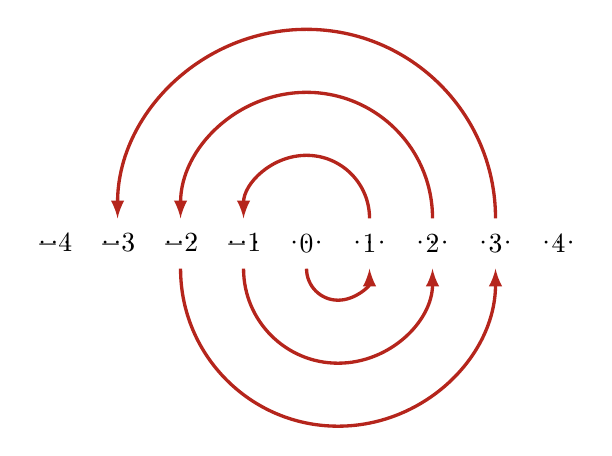
\begin{tikzpicture}[scale=0.8]
            \foreach \x in {-4, ..., 4} {
                \ifthenelse{\x=4 \OR \x=-4}{
                    \node at (\x,0) {\(\cdots\)};
                }{
                    \node at (\x,0) {\(\x\)};
                }
            }

            \foreach \x in {1, 2, 3} {
                \draw[-latex, very thick, BrickRed] (1-\x, -0.4) arc (180:360:\x-0.5);

                \draw[-latex, very thick, BrickRed] (\x, 0.4) arc (0:180:\x);
            }
        \end{tikzpicture}
        \caption{Counting through the set of integers.}
        \label{fig:ch3-counting-through-z}
    \end{figure}

    
    \item \textbf{\(\mathbb{N} \times \mathbb{N}\) is countable.}

    \begin{proof}
        Arrange the ordered pairs \((m, n)\) where \(m, n \in \mathbb{N}\) in a table like so.

        \begin{figure}[H]
            \centering
            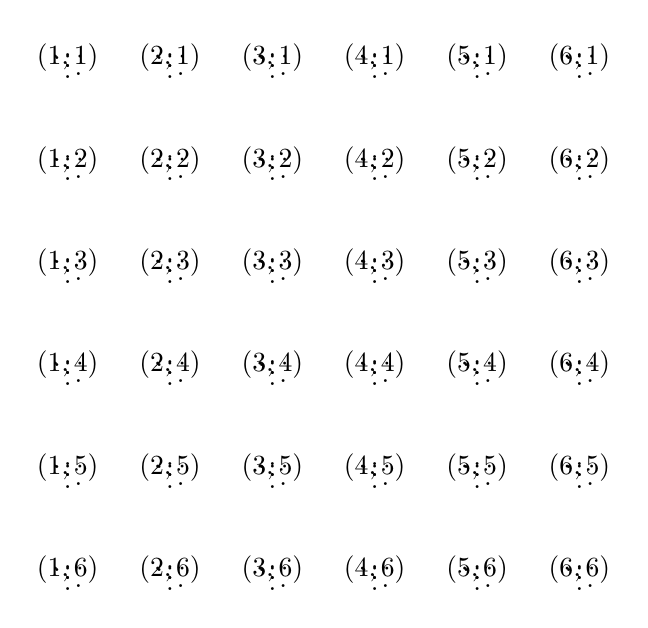
\begin{tikzpicture}[scale=1.3]
                \foreach \x in {1, ..., 6} {
                    \foreach \y in {1, ..., 6} {
                        \ifthenelse{\x=6 \AND \y=6}{
                            \node at (\x,-\y) {\(\ddots\)};
                        }{
                            \ifthenelse{\x=6}{
                                \node at (\x,-\y) {\(\cdots\)};
                            }{
                                \ifthenelse{\y=6}{
                                    \node at (\x,-\y) {\(\vdots\)};
                                }{
                                    \node at (\x,-\y) {\((\x,\y)\)};
                                }
                            }
                        }
                    }
                }
            \end{tikzpicture}
            \caption{A grid of ordered pairs \((m, n)\) where \(m, n \in \mathbb{N}\).}
            \label{fig:ch3-grid-of-ordered-pairs}
        \end{figure}

        We can then count them as follows.

        \begin{figure}[H]
            \centering
            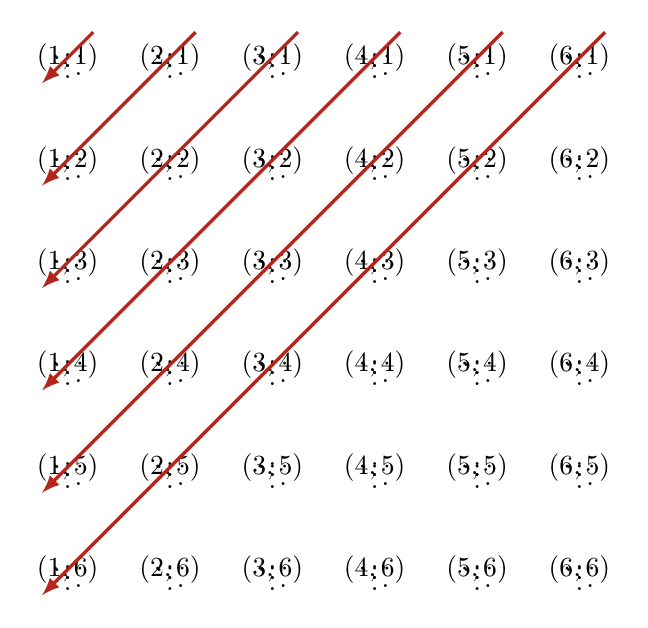
\begin{tikzpicture}[scale=1.3]
                \foreach \x in {1, ..., 6} {
                    \foreach \y in {1, ..., 6} {
                        \ifthenelse{\x=6 \AND \y=6}{
                            \node at (\x,-\y) {\(\ddots\)};
                        }{
                            \ifthenelse{\x=6}{
                                \node at (\x,-\y) {\(\cdots\)};
                            }{
                                \ifthenelse{\y=6}{
                                    \node at (\x,-\y) {\(\vdots\)};
                                }{
                                    \node at (\x,-\y) {\((\x,\y)\)};
                                }
                            }
                        }
                    }
                }

                \foreach \i in {1, ..., 6} {
                    \draw[BrickRed, very thick, -latex] (\i + 0.25, -1+0.25) -- (1-0.25, -\i-0.25);
                }
            \end{tikzpicture}
            \caption{Counting through ordered pairs of natural numbers.}
            \label{fig:ch3-counting-through-ordered-pairs}\qedhere
        \end{figure}
    \end{proof}

    The same argument above can be modified to show that the set of rational numbers \(\mathbb{Q}\) is countable.
\end{enumerate}

Note that not all infinite sets are countable. The set of real numbers, for example, is uncountable as its cardinality exceeds \(\aleph_0\).